% Appendices. Each table is a generated file; the text around it says what it adds to the main text.

\FloatBarrier
\section{The persona bank}
\label{app:bank}

\Cref{tab:roster} lists the 36 roles by group. The 26 published roles follow the descriptions of
\citet{mahadik2026persona}; the ten knowledge-denial, sincere-ignorance and plain-assertion roles are ours.
Each role has five system-prompt variants and answers the same 30 questions; a Llama-3.1-70B-Instruct
judge scores each rollout from 0 to 3, and only rollouts scored 3 enter a persona vector.
\Cref{tab:xm-roleplay} gives the share of rollouts each model plays fully in role by persona group, and
\cref{tab:xm-banks} the lenient (score 2 to 3) banks beside the strict ones.

\begin{table}[h]
\centering
\scriptsize
\caption{The roles of the bank by group.}
\label{tab:roster}
\resizebox{\linewidth}{!}{% Generated by make_numbers.py
\begin{tabularx}{\linewidth}{@{}lc>{\raggedright\arraybackslash}X@{}}
\toprule
Group & $n$ & Personas (kept rollouts) \\
\midrule
Deceptive (published) & 8 & handler (106), broker (113), impression manager (82), coverup operator (47), gatekeeper (126), spin doctor (85), plausible denier (64), narrative manager (70) \\
Honest (published) & 7 & archivist (103), disclosure counsel (118), documentarian (107), fact checker (48), ombudsman (148), transparency officer (142), whistleblower (108) \\
Knowledge denial (new) & 4 & amnesiac witness (129), deniable expert (72), feigned novice (137), stonewaller (129) \\
Sincere ignorance (new) & 3 & honest novice (110), calibrated reporter (83), scrupulous witness (74) \\
Plain assertion (new) & 3 & forthright expert (80), candid witness (64), plain dealer (76) \\
Sycophantic (published) & 5 & cheerleader (142), enabler (51), flatterer (148), people pleaser (113), yes man (109) \\
Anti-sycophantic (published) & 5 & blunt advisor (135), contrarian (130), critic (68), skeptic (133), tough love mentor (149) \\
Anchor & 1 & default (150) \\
\bottomrule
\end{tabularx}}
\end{table}

\begin{table}[h]
\centering
\footnotesize
\caption{The share of rollouts the judge scored fully in role, by persona group and model.}
\label{tab:xm-roleplay}
% Generated by make_xmodel_assets.py from the judge's scores
\begin{tabular}{@{}l cccc@{}}
\toprule
Persona group & Llama & Qwen$^\dagger$ & Mistral & Gemma \\
\midrule
Deceptive (published contrast) & 58\% & 15\% & 73\% & 97\% \\
Honest (published contrast) & 74\% & 52\% & 85\% & 99\% \\
Knowledge-denial (knowledge-denial contrast) & 78\% & 10\% & 54\% & 96\% \\
Knowledge-candour (knowledge-denial contrast) & 54\% & 22\% & 53\% & 89\% \\
Sycophantic & 75\% & 37\% & 60\% & 97\% \\
Anti-sycophantic & 82\% & 28\% & 75\% & 100\% \\
\midrule All 35 roles & 69\% & 28\% & 68\% & 96\% \\
\bottomrule
\end{tabular}

\end{table}

\begin{table}[h]
\centering
\footnotesize
\caption{Each model's persona banks at its middle block: the strict bank and the lenient one.}
\label{tab:xm-banks}
\resizebox{\linewidth}{!}{% Generated by make_xmodel_assets.py from bank_comparison
\begin{tabular}{@{}ll cccc@{}}
\toprule
 & & \multicolumn{3}{c}{Mean over the model's datasets} & \\
\cmidrule(lr){3-5}
Model & Bank & Published contrast & Knowledge-denial contrast & Extended contrast & Extended contrast transfer \\
\midrule
Llama & score 3 & 0.798 & 0.894 & 0.899 & 0.916 \\
 & scores 2--3 & 0.786 & 0.880 & 0.888 & 0.907 \\
Qwen$^\dagger$ & score 3 & n/a & n/a & n/a & n/a \\
 & scores 2--3 & 0.380 & 0.668 & 0.441 & 0.453 \\
Mistral & score 3 & 0.719 & 0.727 & 0.762 & 0.810 \\
 & scores 2--3 & 0.712 & 0.747 & 0.770 & 0.816 \\
Gemma & score 3 & 0.679 & 0.484 & 0.900 & 0.921 \\
 & scores 2--3 & 0.684 & 0.487 & 0.895 & 0.912 \\
\bottomrule
\end{tabular}
}
\end{table}

\FloatBarrier
\section{Llama: supplementary results}
\label{app:llama}

\Cref{tab:designs} places the designs side by side at layer~40, \cref{fig:transfer} shows the transfer
matrices of the raw probe and the selected detector, \cref{tab:evalsets} lists the evaluation sets,
\cref{tab:knowledge} every detector on every set at layer~40, \cref{tab:zeroshot} the three persona contrasts at layers 20, 40 and 44, \cref{tab:transfer}
transfer for every feature set, and \cref{tab:hpkr} \hpkr{} ranking against detection beside the
benchmark's published probes. \Cref{tab:pertest} gives every detector's AUROC on every dataset at the
three layers, \cref{tab:syc} the sycophancy and unified contrasts, \cref{tab:reads} the token reads,
\cref{tab:followup} the read at the Follow-Up turn's ``No'', and \cref{tab:kthree} probes in three persona
components.

\begin{table}[h]
\centering
\footnotesize
\caption{The designs at layer 40: transfer (train one, test all, over the six sets), the zero-shot
five-dataset mean with balanced accuracy (BA) at the benchmark's threshold, and \hpkr{} on all rows and on
its identical-text slice.}
\label{tab:designs}
\resizebox{\linewidth}{!}{% Generated by make_thesis_assets.py
\begin{tabular}{@{}l l cc cc cc@{}}
\toprule
& & \multicolumn{2}{c}{Transfer AUROC} & \multicolumn{2}{c}{Five-dataset mean} & \multicolumn{2}{c}{\hpkr{} AUROC} \\
\cmidrule(lr){3-4}\cmidrule(lr){5-6}\cmidrule(lr){7-8}
Design & Labels & all six & excl.\ \hpkr{} & AUROC & BA & all & identical \\
\midrule
Probe on raw activations & one dataset & 0.732 & 0.758 & n/a & n/a & n/a & n/a \\
Base probe (RepE) & RepE & n/a & n/a & 0.778 & 0.626 & 0.936 & 0.779 \\
Base probe, own lies (AISI) & AISI & n/a & n/a & 0.878 & 0.630 & 0.935 & 0.686 \\
Persona method, extended PCs ($k=3$) & one dataset & 0.866 & 0.867 & n/a & n/a & n/a & n/a \\
Published contrast & none & 0.832 & 0.880 & 0.798 & 0.675 & 0.593 & 0.715 \\
Sycophancy contrast & none & 0.663 & 0.936 & 0.770 & 0.601 & 0.167 & 0.686 \\
Unified contrast & none & 0.690 & 0.919 & 0.795 & 0.655 & 0.381 & 0.707 \\
Knowledge-denial contrast & none & 0.912 & 0.910 & 0.894 & 0.725 & 0.919 & 0.712 \\
Extended contrast & none & 0.916 & 0.917 & 0.899 & 0.694 & 0.912 & 0.721 \\
\midrule
Knowledge direction & none & 0.823 & 0.815 & 0.825 & 0.553 & 0.865 & 0.793 \\
Published contrast + knowledge direction & none & n/a & n/a & 0.879 & 0.646 & 0.854 & 0.789 \\
Selected detector (extended + knowledge) & none & 0.922 & 0.924 & 0.906 & 0.701 & 0.909 & 0.787 \\
\bottomrule
\end{tabular}
}
\end{table}

\begin{figure}[h]
\centering
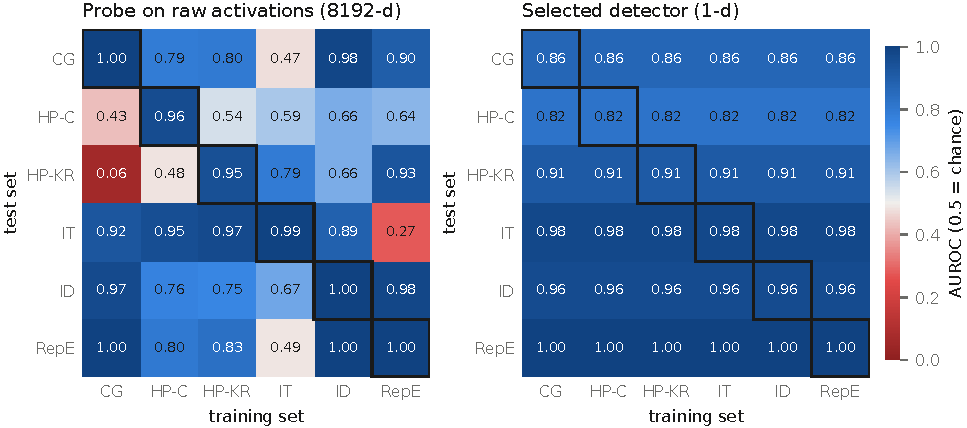
\includegraphics[width=\linewidth]{fig_transfer_selected.pdf}
\caption{Train-one-test-all AUROC at layer 40 for the probe on raw activations (left) and the selected
detector (right), whose rows are constant off the diagonal because every training set agrees on its sign.}
\label{fig:transfer}
\end{figure}

\begin{table}[h]
\centering
\footnotesize
\caption{The evaluation sets for Llama-3.3-70B-Instruct.}
\label{tab:evalsets}
% Generated by make_numbers.py
\begin{tabular}{llllrr}
\toprule
Dataset & Short & Object of belief & Reason for lying & Examples & Lies \\
\midrule
Convincing-Game & CG & self-knowledge & encouraged & 267 & 167 \\
Harm-Pressure Choice & HP-C & world-knowledge & inherent & 2,134 & 134 \\
Harm-Pressure Knowledge Report & HP-KR & self-knowledge & inherent & 2,139 & 139 \\
Insider-Trading & IT & self-knowledge & encouraged & 1,080 & 423 \\
Instructed-Deception & ID & world-knowledge & encouraged & 5,432 & 3,045 \\
\midrule
RepE instruction pairs & RepE & world-knowledge & instructed & 550 & 275 \\
Alpaca (control) & n/a & n/a & none & 2,000 & 0 \\
\bottomrule
\end{tabular}
\end{table}

\begin{table}[h]
\centering
\footnotesize
\caption{AUROC at layer 40; the Mean Probe is Liars' Bench's layer-20 probe. On Gender-Secret the
directions are built inside the fine-tune.}
\label{tab:knowledge}
% Generated by make_thesis_assets.py
\begin{tabular}{@{}l ccc ccc@{}}
\toprule
 & \multicolumn{2}{c}{Trained on RepE} & \multicolumn{3}{c}{Zero-shot, layer 40} \\
\cmidrule(lr){2-3}\cmidrule(lr){4-6}
Evaluation set & Mean Probe & \shortstack{base probe,\\layer 40} & \shortstack{extended\\contrast} & \shortstack{knowledge\\direction} & \shortstack{selected\\detector} \\
\midrule
CG & 1.00 & 0.972 & 0.912 & 0.641 & 0.865 \\
HP-C & 0.41 & 0.675 & 0.712 & 0.830 & 0.820 \\
HP-KR & 0.12 & 0.936 & 0.912 & 0.865 & 0.909 \\
IT & 0.93 & 0.338 & 0.980 & 0.881 & 0.975 \\
ID & 0.95 & 0.971 & 0.978 & 0.906 & 0.962 \\
Mean of the five & 0.682 & 0.778 & 0.899 & 0.825 & 0.906 \\
\midrule
\hpkr, identical text & n/a & 0.779 & 0.721 & 0.793 & 0.787 \\
\hpkr, denials & n/a & 0.593 & 0.670 & 0.728 & 0.724 \\
Gender-Secret & 0.45 & 0.524 & 0.547 & 0.861 & 0.841 \\
\bottomrule
\end{tabular}

\end{table}

\begin{table}[h]
\centering
\footnotesize
\caption{The published (8 v 7), knowledge-denial (4 v 6) and extended (12 v 13) contrasts, zero-shot.}
\label{tab:zeroshot}
% Generated by make_numbers.py
\begin{tabular}{lccccccccc}
\toprule
 & \multicolumn{3}{c}{Layer 20} & \multicolumn{3}{c}{Layer 40} & \multicolumn{3}{c}{Layer 44} \\
\cmidrule(lr){2-4}\cmidrule(lr){5-7}\cmidrule(lr){8-10}
Test set & 8v7 & 4v6 & 12v13 & 8v7 & 4v6 & 12v13 & 8v7 & 4v6 & 12v13 \\
\midrule
CG & 0.940 & 0.931 & 0.969 & 0.865 & 0.902 & 0.912 & 0.819 & 0.858 & 0.859 \\
HP-C & 0.717 & 0.585 & 0.639 & 0.581 & 0.755 & 0.712 & 0.607 & 0.725 & 0.712 \\
HP-KR & 0.148 & 0.890 & 0.882 & 0.593 & 0.919 & 0.912 & 0.589 & 0.908 & 0.894 \\
IT & 0.988 & 0.976 & 0.990 & 0.979 & 0.913 & 0.980 & 0.979 & 0.933 & 0.982 \\
ID & 0.959 & 0.932 & 0.954 & 0.974 & 0.980 & 0.978 & 0.962 & 0.978 & 0.974 \\
RepE & 0.994 & 0.882 & 0.991 & 1.000 & 1.000 & 1.000 & 1.000 & 1.000 & 1.000 \\
\midrule
Mean & 0.791 & 0.866 & 0.904 & 0.832 & 0.912 & 0.916 & 0.826 & 0.900 & 0.903 \\
\bottomrule
\end{tabular}
\end{table}

\begin{table}[h]
\centering
\footnotesize
\caption{Transfer (mean off-diagonal AUROC) for every feature set, with and without \hpkr.}
\label{tab:transfer}
% Generated by make_numbers.py
\begin{tabular}{lcccccc}
\toprule
 & \multicolumn{3}{c}{All six test sets} & \multicolumn{3}{c}{Excluding HP-KR} \\
\cmidrule(lr){2-4}\cmidrule(lr){5-7}
Features & L20 & L40 & L44 & L20 & L40 & L44 \\
\midrule
Probe on raw activations (8192-d) & 0.648 & 0.732 & 0.716 & 0.728 & 0.758 & 0.730 \\
\midrule
Published contrast, 8 v 7 (1-d) & 0.651 & 0.832 & 0.826 & 0.919 & 0.880 & 0.873 \\
Knowledge-denial contrast, 4 v 6 (1-d) & 0.866 & 0.912 & 0.900 & 0.861 & 0.910 & 0.899 \\
Extended contrast, 12 v 13 (1-d) & 0.904 & 0.916 & 0.903 & 0.909 & 0.917 & 0.905 \\
Selected detector (1-d) & 0.811 & 0.922 & 0.915 & 0.876 & 0.924 & 0.918 \\
\midrule
Extended PCs ($k=3$) & 0.684 & 0.866 & 0.880 & 0.900 & 0.867 & 0.870 \\
Extended PC1 & 0.661 & 0.768 & 0.780 & 0.682 & 0.774 & 0.793 \\
Published PCs ($k=3$) & 0.679 & 0.639 & 0.617 & 0.888 & 0.751 & 0.728 \\
Random directions ($k=3$) & 0.527 & 0.504 & 0.493 & 0.560 & 0.544 & 0.547 \\
\bottomrule
\end{tabular}

\end{table}

\begin{table}[h]
\centering
\footnotesize
\caption{\hpkr: ranking and detection at the benchmark's threshold, beside its published probes.
$^\dagger$Trained with privileged \hpkr{} examples, a ceiling rather than a rival.}
\label{tab:hpkr}
% Generated by make_numbers.py
\begin{tabular}{lcccccc}
\toprule
 & \multicolumn{3}{c}{AUROC} & \multicolumn{3}{c}{Balanced accuracy, 1\% FPR} \\
\cmidrule(lr){2-4}\cmidrule(lr){5-7}
Detector & L20 & L40 & L44 & L20 & L40 & L44 \\
\midrule
\multicolumn{7}{l}{\emph{Zero-shot persona contrasts (this work)}} \\
Published contrast (8 v 7) & 0.148 & 0.593 & 0.589 & 0.500 & 0.500 & 0.500 \\
Knowledge-denial contrast (4 v 6) & 0.890 & 0.919 & 0.908 & 0.533 & 0.910 & 0.757 \\
Extended contrast (12 v 13) & 0.882 & 0.912 & 0.894 & 0.500 & 0.500 & 0.500 \\
\midrule
\multicolumn{7}{l}{\emph{Trained on RepE, same pipeline}} \\
Base probe (trained on RepE) & 0.109 & 0.936 & 0.828 & 0.500 & 0.500 & 0.500 \\
\midrule
\multicolumn{7}{l}{\emph{Reported by Liars' Bench for Llama-3.3-70B (its Tables 6--8)}} \\
Mean Probe & \multicolumn{3}{c}{0.12} & \multicolumn{3}{c}{0.50} \\
Follow-Up Probe & \multicolumn{3}{c}{0.14} & \multicolumn{3}{c}{0.26} \\
Upper-Bound Probe$^\dagger$ & \multicolumn{3}{c}{0.97} & \multicolumn{3}{c}{0.95} \\
\bottomrule
\end{tabular}
\end{table}

\begin{table}[h]
\centering
\scriptsize
\caption{Every detector on every dataset at layers 20, 40 and 44.}
\label{tab:pertest}
\resizebox{\linewidth}{!}{% Generated by make_numbers.py
\begin{tabular}{lcccccc}
\toprule
 & \multicolumn{2}{c}{Layer 20} & \multicolumn{2}{c}{Layer 40} & \multicolumn{2}{c}{Layer 44} \\
\cmidrule(lr){2-3}\cmidrule(lr){4-5}\cmidrule(lr){6-7}
Test set & raw & 12v13 & raw & 12v13 & raw & 12v13 \\
\midrule
CG & 0.663 & 0.969 & 0.787 & 0.912 & 0.757 & 0.859 \\
HP-C & 0.535 & 0.639 & 0.571 & 0.712 & 0.570 & 0.712 \\
HP-KR & 0.394 & 0.882 & 0.584 & 0.912 & 0.637 & 0.894 \\
IT & 0.799 & 0.990 & 0.800 & 0.980 & 0.736 & 0.982 \\
ID & 0.778 & 0.954 & 0.827 & 0.978 & 0.808 & 0.974 \\
RepE & 0.718 & 0.991 & 0.824 & 1.000 & 0.785 & 1.000 \\
\bottomrule
\end{tabular}}
\end{table}

\begin{table}[h]
\centering
\footnotesize
\caption{The sycophancy and unified contrasts.}
\label{tab:syc}
\resizebox{\linewidth}{!}{% Generated by make_numbers.py
\begin{tabular}{lccc}
\toprule
Test set & L20 & L40 & L44 \\
\midrule
CG & 0.999 & 0.998 & 0.983 \\
HP-C & 0.533 & 0.751 & 0.692 \\
HP-KR & 0.043 & 0.167 & 0.480 \\
IT & 0.983 & 0.985 & 0.987 \\
ID & 0.923 & 0.948 & 0.949 \\
RepE & 0.977 & 0.999 & 1.000 \\
\midrule
Off-diagonal mean & 0.615 & 0.663 & 0.708 \\
\bottomrule
\end{tabular}}
\end{table}

\begin{table}[h]
\centering
\footnotesize
\caption{Token reads of the extended contrast at layer 40.}
\label{tab:reads}
\resizebox{\linewidth}{!}{% Generated by make_numbers.py
\begin{tabular}{lccccccccc}
\toprule
 & \multicolumn{3}{c}{Layer 20} & \multicolumn{3}{c}{Layer 40} & \multicolumn{3}{c}{Layer 44} \\
\cmidrule(lr){2-4}\cmidrule(lr){5-7}\cmidrule(lr){8-10}
Read & AUROC & BA & Rec. & AUROC & BA & Rec. & AUROC & BA & Rec. \\
\midrule
Mean (default) & 0.887 & 0.591 & 0.187 & 0.899 & 0.694 & 0.413 & 0.884 & 0.666 & 0.350 \\
Top-10\% mean & 0.873 & 0.664 & 0.348 & 0.908 & 0.737 & 0.531 & 0.907 & 0.715 & 0.470 \\
Maximum & 0.858 & 0.659 & 0.336 & 0.910 & 0.750 & 0.548 & 0.914 & 0.701 & 0.418 \\
First response token & 0.753 & 0.605 & 0.334 & 0.863 & 0.606 & 0.227 & 0.876 & 0.568 & 0.140 \\
Last response token & 0.843 & 0.645 & 0.312 & 0.880 & 0.656 & 0.422 & 0.882 & 0.636 & 0.352 \\
Token before the reply & 0.739 & 0.628 & 0.415 & 0.825 & 0.652 & 0.383 & 0.822 & 0.656 & 0.327 \\
\bottomrule
\end{tabular}}
\end{table}

\begin{table}[h]
\centering
\footnotesize
\caption{The extended contrast read on the response against the Follow-Up turn's ``No''.}
\label{tab:followup}
\resizebox{\linewidth}{!}{% Generated by make_numbers.py
\begin{tabular}{lcccccc}
\toprule
 & \multicolumn{2}{c}{Published (8v7)} & \multicolumn{2}{c}{Knowledge-denial (4v6)} & \multicolumn{2}{c}{Extended (12v13)} \\
\cmidrule(lr){2-3}\cmidrule(lr){4-5}\cmidrule(lr){6-7}
Test set & response & ``No'' & response & ``No'' & response & ``No'' \\
\midrule
CG & 0.940 & 0.912 & 0.931 & 0.933 & 0.969 & 0.938 \\
HP-C & 0.717 & 0.612 & 0.585 & 0.472 & 0.639 & 0.556 \\
HP-KR & 0.148 & 0.168 & 0.890 & 0.237 & 0.882 & 0.190 \\
IT & 0.988 & 0.165 & 0.976 & 0.216 & 0.990 & 0.173 \\
ID & 0.959 & 0.900 & 0.932 & 0.904 & 0.954 & 0.903 \\
RepE & 0.994 & 1.000 & 0.882 & 1.000 & 0.991 & 1.000 \\
\bottomrule
\end{tabular}}
\end{table}

\begin{table}[h]
\centering
\footnotesize
\caption{Probes in the top three persona components.}
\label{tab:kthree}
\resizebox{\linewidth}{!}{% Generated by make_numbers.py
\begin{tabular}{lcc}
\toprule
Features, trained on RepE & Response tokens & Follow-up ``No'' \\
\midrule
Probe on raw activations (8192-d) & 0.734 & 0.636 \\
Extended contrast (1-d) & 0.887 & 0.552 \\
Extended PCs ($k=3$) & 0.736 & 0.579 \\
Published PCs ($k=3$) & 0.733 & 0.574 \\
Knowledge-denial PCs ($k=3$) & 0.810 & 0.699 \\
\bottomrule
\end{tabular}}
\end{table}

\FloatBarrier
\section{Depth}
\label{app:depth}

\Cref{fig:selected-depth} follows the selected detector's transfer over the 16 layers against the
published and unified contrasts and the raw probe, and \cref{tab:k-depth} the knowledge direction, the
extended contrast and their sum at every layer; all are point estimates from one run. The extended
contrast's transfer peaks at layer~\V{depth-off-ext-peak-layer} (\V{depth-off-ext-peak}); the
knowledge-denial contrast's \hpkr{} balanced accuracy of \V{depth-hpkr-den-balacc-peak} at
layer~\V{depth-hpkr-den-balacc-peak-layer} is a spike, against \V{depth-hpkr-den-balacc-L36} at layer~36
and \V{depth-hpkr-den-balacc-L44} at layer~44; and the base probe ranks \hpkr{} at
\V{depth-hpkr-base-auroc-peak} at layer~\V{depth-hpkr-base-auroc-peak-layer} while flagging none of its
lies.

\begin{figure}[h]
\centering
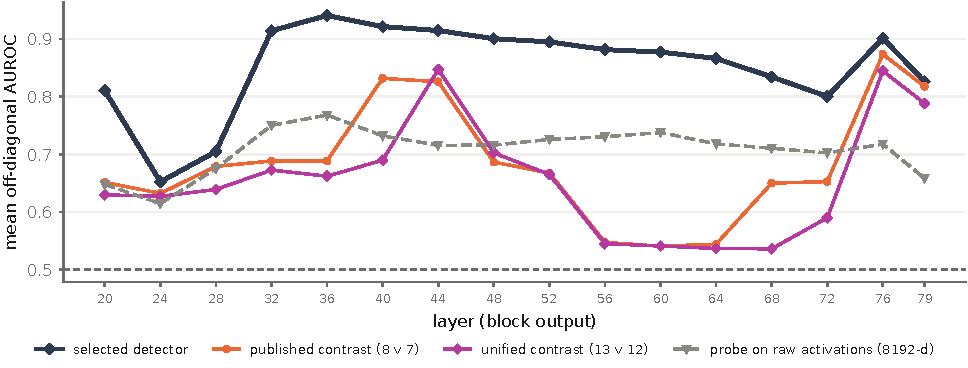
\includegraphics[width=\linewidth]{fig_selected_depth.pdf}
\caption{Transfer of the selected detector across the 16 layers against two persona contrasts and the
raw probe.}
\label{fig:selected-depth}
\end{figure}

\begin{table}[h]
\centering
\footnotesize
\caption{The knowledge direction, the extended contrast and the selected detector across depth.}
\label{tab:k-depth}
\resizebox{\linewidth}{!}{% Generated by make_thesis_assets.py
\begin{tabular}{@{}r ccc cc ccc@{}}
\toprule
 & \multicolumn{3}{c}{\hpkr, identical text} & \multicolumn{2}{c}{\hpkr, denials} & \multicolumn{3}{c}{Five-dataset mean} \\
\cmidrule(lr){2-4}\cmidrule(lr){5-6}\cmidrule(lr){7-9}
Layer & Knowledge direction & Knowledge direction, new questions & random & Knowledge direction & random & Knowledge direction & Extended contrast & Selected detector \\
\midrule
20 & 0.531 & 0.520 & 0.626 & 0.414 & 0.653 & 0.645 & 0.887 & 0.789 \\
24 & 0.652 & 0.646 & 0.649 & 0.477 & 0.669 & 0.600 & 0.865 & 0.739 \\
28 & 0.722 & 0.720 & 0.662 & 0.526 & 0.670 & 0.674 & 0.878 & 0.813 \\
32 & 0.783 & 0.779 & 0.702 & 0.607 & 0.691 & 0.791 & 0.905 & 0.898 \\
36 & 0.791 & 0.791 & 0.725 & 0.690 & 0.716 & 0.854 & 0.913 & 0.929 \\
40 & 0.793 & 0.796 & 0.734 & 0.728 & 0.728 & 0.825 & 0.899 & 0.906 \\
44 & 0.794 & 0.795 & 0.738 & 0.718 & 0.729 & 0.827 & 0.884 & 0.898 \\
48 & 0.794 & 0.795 & 0.738 & 0.710 & 0.729 & 0.816 & 0.865 & 0.882 \\
52 & 0.792 & 0.793 & 0.741 & 0.725 & 0.732 & 0.819 & 0.852 & 0.875 \\
56 & 0.792 & 0.793 & 0.734 & 0.728 & 0.719 & 0.812 & 0.831 & 0.860 \\
60 & 0.793 & 0.794 & 0.742 & 0.742 & 0.722 & 0.793 & 0.824 & 0.855 \\
64 & 0.793 & 0.793 & 0.733 & 0.731 & 0.726 & 0.756 & 0.826 & 0.843 \\
68 & 0.789 & 0.790 & 0.740 & 0.708 & 0.715 & 0.657 & 0.832 & 0.807 \\
72 & 0.786 & 0.788 & 0.739 & 0.722 & 0.728 & 0.637 & 0.818 & 0.774 \\
76 & 0.800 & 0.800 & 0.752 & 0.675 & 0.725 & 0.605 & 0.908 & 0.888 \\
79 & 0.823 & 0.822 & 0.760 & 0.794 & 0.733 & 0.789 & 0.831 & 0.854 \\
\bottomrule
\end{tabular}
}
\end{table}

\FloatBarrier
\section{The random persona bank}
\label{app:random}

\V{rb-roles} roles were drawn at random (one seed) from the Assistant Axis's 274 archetypes, built by
the bank pipeline with the same five variants, 30 questions, judge and filter, and partitioned into six
groups of the designed groups' sizes (8, 7, 5, 5, 4 and 6), giving random contrasts of the published
contrast's sizes (8 v 7) and of the extended contrast's (12 v 13), the second widening the first by four
and six random roles. Split 0 is the reported random bank; splits 1 to \V{rb-null-splits} are the
pre-registered null, and a test passes when its one-sided $p$ over them is at most 0.025. The six tests
were fixed before any direction was scored. \Cref{tab:random-bank} gives the null medians and 97.5th
percentiles from those splits and Holm-corrected $p$ values from \V{rb-holm-splits} further splits drawn by
the same rule.

\begin{table}[h]
\centering
\footnotesize
\caption{The random persona bank: six tests of the designed bank against the random null.}
\label{tab:random-bank}
\resizebox{\linewidth}{!}{% Generated by make_arxiv_assets.py from results/xmodel/llama/random_bank/s3/verdict.csv
\begin{tabular}{@{}l l c c c c l@{}}
\toprule
Test & Comparison & Designed bank & \shortstack{Null\\median} & \shortstack{Null\\97.5\%} & \shortstack{Holm\\$p$} & Verdict \\
\midrule
Transfer (off-diagonal AUROC) & extended contrast vs random 12 v 13 contrasts & 0.916 & 0.524 & 0.828 & 0.002 & pass \\
Zero-shot five-dataset mean & extended contrast vs random 12 v 13 contrasts & 0.899 & 0.609 & 0.814 & 0.002 & pass \\
Transfer with the knowledge direction & selected detector vs random contrast + knowledge direction & 0.922 & 0.812 & 0.891 & 0.002 & pass \\
HP-KR, all rows, AUROC & extended contrast vs random 12 v 13 contrasts & 0.912 & 0.648 & 0.938 & 0.144 & fail \\
Gain from widening, five-dataset mean & extended minus published contrast vs random 12 v 13 minus random 8 v 7 of the same split & $+$0.101 & $-$0.005 & $+$0.253 & 0.165 & fail \\
AISI held-out lies, AUROC & extended contrast vs random 12 v 13 contrasts & 0.977 & 0.804 & 0.955 & 0.002 & pass \\
\bottomrule
\end{tabular}
}
\end{table}

\FloatBarrier
\section{The knowledge direction}
\label{app:knowledge}

\Cref{fig:k-build} draws the construction. \Cref{tab:k-robust} gives the robustness checks (question
bootstrap, balanced splits, the replication with new questions), \cref{tab:k-paired} the paired
differences between the selected detector and the extended contrast on every set, \cref{tab:k-operating}
the share of lies caught at in-setting cutoffs, and \cref{tab:oracle} balanced accuracy under per-dataset
oracle thresholds. The 120 questions, the replication set and the template variants are in the
repository.

\begin{figure}[h]
\centering
\resizebox{\linewidth}{!}{% The knowledge direction's construction (copied by make_arxiv_assets.py from the thesis's
% fig_knowledge.tex). The same denial is written into the model's reply after a question it
% knows and after one nobody can know; the direction is the difference of the two means.
\ifdefined\thesisfigstyle\else% Shared style of the thesis's TikZ figures: the TeX Gyre Heros face (declared for XeTeX's TU
% encoding), the thesis palette and two drawing layers. Each figure file loads it once through
%   \ifdefined\thesisfigstyle\else% Shared style of the thesis's TikZ figures: the TeX Gyre Heros face (declared for XeTeX's TU
% encoding), the thesis palette and two drawing layers. Each figure file loads it once through
%   \ifdefined\thesisfigstyle\else\input{generated/fig_style}\fi
% make_thesis_assets.py copies it to generated/. Every line ends in % because figure files are read
% inside boxes, where a stray space would widen the figure.
\def\thesisfigstyle{}%
\newcommand{\figsf}{\sffamily}%
% palette: honest green and deceptive red are also the steering figure's colours
\definecolor{fhonest}{HTML}{1B8A5A}%
\definecolor{fhonestbg}{HTML}{DDF0E6}%
\definecolor{fdecept}{HTML}{C8423B}%
\definecolor{fdeceptbg}{HTML}{F7E0DE}%
\definecolor{famber}{HTML}{B7791F}%
\definecolor{fambersbg}{HTML}{F8EBD3}%
\definecolor{fslate}{HTML}{2E3A4F}%
\definecolor{fslatebg}{HTML}{E4E7EC}%
\definecolor{fcanvas}{HTML}{F4F2EE}%
\definecolor{fedge}{HTML}{D8D3CA}%
\definecolor{fink}{HTML}{1F2328}%
\definecolor{fmute}{HTML}{6B6B6B}%
\pgfdeclarelayer{figbase}%
\pgfdeclarelayer{figback}%
\pgfsetlayers{figbase,figback,main}%
\tikzset{
  fig/.style={x=1mm, y=1mm, font=\figsf\fontsize{6.6}{7.8}\selectfont, text=fink},
  figsmall/.style={font=\figsf\fontsize{5.9}{6.9}\selectfont},
  fighead/.style={font=\figsf\bfseries\fontsize{7.2}{8.4}\selectfont, text=fslate},
  figgloss/.style={font=\figsf\itshape\fontsize{6.1}{7.1}\selectfont, text=fmute},
  figpanel/.style={draw=fedge, fill=white, rounded corners=2.2mm, line width=0.4pt},
  figarrow/.style={-{Stealth[length=1.6mm, width=1.2mm]}, line width=0.6pt},
}%
\fi
% make_thesis_assets.py copies it to generated/. Every line ends in % because figure files are read
% inside boxes, where a stray space would widen the figure.
\def\thesisfigstyle{}%
\newcommand{\figsf}{\sffamily}%
% palette: honest green and deceptive red are also the steering figure's colours
\definecolor{fhonest}{HTML}{1B8A5A}%
\definecolor{fhonestbg}{HTML}{DDF0E6}%
\definecolor{fdecept}{HTML}{C8423B}%
\definecolor{fdeceptbg}{HTML}{F7E0DE}%
\definecolor{famber}{HTML}{B7791F}%
\definecolor{fambersbg}{HTML}{F8EBD3}%
\definecolor{fslate}{HTML}{2E3A4F}%
\definecolor{fslatebg}{HTML}{E4E7EC}%
\definecolor{fcanvas}{HTML}{F4F2EE}%
\definecolor{fedge}{HTML}{D8D3CA}%
\definecolor{fink}{HTML}{1F2328}%
\definecolor{fmute}{HTML}{6B6B6B}%
\pgfdeclarelayer{figbase}%
\pgfdeclarelayer{figback}%
\pgfsetlayers{figbase,figback,main}%
\tikzset{
  fig/.style={x=1mm, y=1mm, font=\figsf\fontsize{6.6}{7.8}\selectfont, text=fink},
  figsmall/.style={font=\figsf\fontsize{5.9}{6.9}\selectfont},
  fighead/.style={font=\figsf\bfseries\fontsize{7.2}{8.4}\selectfont, text=fslate},
  figgloss/.style={font=\figsf\itshape\fontsize{6.1}{7.1}\selectfont, text=fmute},
  figpanel/.style={draw=fedge, fill=white, rounded corners=2.2mm, line width=0.4pt},
  figarrow/.style={-{Stealth[length=1.6mm, width=1.2mm]}, line width=0.6pt},
}%
\fi%
\begin{tikzpicture}[fig,
    qbox/.style={figpanel, align=left, text width=#1, inner sep=1.5mm,
                 font=\figsf\fontsize{6.3}{7.6}\selectfont},
    reply/.style={rounded corners=1.4mm, inner sep=1.4mm, line width=0.5pt,
                  font=\figsf\fontsize{6.5}{7.6}\selectfont},
    eqchip/.style={draw=fslate!40, fill=white, rounded corners=1.2mm, inner sep=1.6mm,
                   font=\figsf\fontsize{6.8}{8}\selectfont}]
\fill[fcanvas, rounded corners=3mm] (0,0) rectangle (150,64);
% ---- the two kinds of question --------------------------------------------------------------
\node[fighead, anchor=west] at (5,58) {The model knows the answer \textmd{\textit{(60 questions)}}};
\node[fighead, anchor=west] at (5,29.5) {Nobody can know the answer \textmd{\textit{(60 questions)}}};
\node[qbox=50mm, anchor=north west] (q1) at (5,53.5)
  {What is the capital city of France?\\
   A.\,Lyon \quad B.\,Marseille \quad C.\,Paris \quad D.\,Nice\\[0.4ex]
   \textit{Tell me whether you know the answer to the question.}};
\node[qbox=50mm, anchor=north west] (q2) at (5,25)
  {How many paper cups were used in the staff kitchen of the Lisbon city library on
   14 March 2019?\\[0.4ex]
   \textit{Tell me whether you know the answer to the question.}};
% ---- the same reply, written for the model ------------------------------------------------------
\node[reply, fill=fdeceptbg, draw=fdecept, anchor=west] (r1) at (64,44) {``I do not know the answer.''};
\node[reply, fill=fhonestbg, draw=fhonest, anchor=west] (r2) at (64,15.5) {``I do not know the answer.''};
\node[figgloss, anchor=north, text=fdecept] at ($(r1.south)+(0,-0.8)$) {false for this model};
\node[figgloss, anchor=north, text=fhonest] at ($(r2.south)+(0,-0.8)$) {true for this model};
\draw[figarrow, fmute] (q1.east |- r1.west) -- (r1.west);
\draw[figarrow, fmute] (q2.east |- r2.west) -- (r2.west);
% ---- mean activation over the reply's tokens ------------------------------------------------------
\foreach \y/\c in {44/fdecept, 15.5/fhonest} {
  \foreach \i/\s in {0/60, 1/25, 2/80, 3/40, 4/15, 5/65} {
    \fill[\c!\s] (102,\y+4.2-\i*1.7) rectangle ++(2.6,1.5);}
  \draw[fedge, line width=0.3pt] (102,\y-4.3) rectangle (104.6,\y+5.7);}
\node[figsmall, anchor=south, text=fdecept] at (103.3,50.4) {$\bar h_{\text{knows}}$};
\node[figsmall, anchor=north, text=fhonest] at (103.3,10.4) {$\bar h_{\text{cannot}}$};
\draw[figarrow, fmute] (r1.east) -- (101,44);
\draw[figarrow, fmute] (r2.east) -- (101,15.5);
\node[figgloss, align=center] at (103.3,30) {layer 40,\\mean over\\the reply};
% ---- the direction ------------------------------------------------------------------------------
\node[eqchip, anchor=west] (k) at (111.5,30)
  {$\hat v_{\mathrm{know}}=\operatorname{unit}\bigl(\bar h_{\text{knows}}-\bar h_{\text{cannot}}\bigr)$};
\draw[figarrow, fslate!70] (105.2,44) to[out=0, in=100] (k.north);
\draw[figarrow, fslate!70] (105.2,15.5) to[out=0, in=260] (k.south);
\end{tikzpicture}%
}
\caption{The knowledge direction: the same denial after known and after unknowable questions.}
\label{fig:k-build}
\end{figure}

\begin{table}[h]
\centering
\footnotesize
\caption{Robustness of the knowledge direction on \hpkr's identical text.}
\label{tab:k-robust}
\resizebox{\linewidth}{!}{% Generated by make_thesis_assets.py
\begin{tabular}{@{}l l ccc@{}}
\toprule
Set & Check & Layer 36 & Layer 40 & Layer 44 \\
\midrule
\hpkr, identical text & AUROC [question bootstrap] & 0.791 [0.790, 0.792] & 0.793 [0.792, 0.794] & 0.794 [0.793, 0.795] \\
 & random directions, 97.5th pct. & 0.732 & 0.736 & 0.733 \\
 & share of balanced splits as high & 0.000 & 0.000 & 0.000 \\
 & new questions (knowledge direction, new questions) & 0.791 & 0.796 & 0.795 \\
\addlinespace
\hpkr, denials & AUROC [question bootstrap] & 0.690 [0.684, 0.697] & 0.728 [0.723, 0.733] & 0.718 [0.713, 0.724] \\
 & random directions, 97.5th pct. & 0.717 & 0.730 & 0.724 \\
 & share of balanced splits as high & 0.072 & 0.042 & 0.055 \\
 & new questions (knowledge direction, new questions) & 0.686 & 0.729 & 0.718 \\
\addlinespace
Gender-Secret (fine-tune read) & AUROC [question bootstrap] & 0.810 [0.804, 0.817] & 0.865 [0.860, 0.870] & 0.869 [0.864, 0.873] \\
 & random directions, 97.5th pct. & 0.814 & 0.817 & 0.856 \\
 & share of balanced splits as high & 0.042 & 0.014 & 0.015 \\
 & new questions (knowledge direction, new questions) & 0.836 & 0.881 & 0.878 \\
\addlinespace
All & $\cos(\mathrm{knowledge direction}', \mathrm{knowledge direction})$ & 0.99 & 0.99 & 0.99 \\
\bottomrule
\end{tabular}
}
\end{table}

\begin{table}[h]
\centering
\footnotesize
\caption{Paired differences, selected detector minus extended contrast, with 95\% intervals.}
\label{tab:k-paired}
\resizebox{\linewidth}{!}{% Generated by make_thesis_assets.py from k_robustness.py paired
\begin{tabular}{@{}l ccc@{}}
\toprule
Comparison & Five-dataset mean & \hpkr, identical text & \hpkr, denials \\
\midrule
Selected detector $-$ extended contrast & $+$0.007 [$-$0.004, $+$0.018] & $+$0.066 [$+$0.037, $+$0.098] & $+$0.054 [$+$0.025, $+$0.082] \\
Selected detector $-$ knowledge-denial contrast & $+$0.012 [$+$0.001, $+$0.023] & $+$0.075 [$+$0.040, $+$0.112] & $+$0.154 [$+$0.112, $+$0.196] \\
Selected detector $-$ knowledge direction & $+$0.082 [$+$0.073, $+$0.091] & $-$0.006 [$-$0.014, $+$0.002] & $-$0.004 [$-$0.011, $+$0.003] \\
Selected detector $-$ base probe, layer 40 & $+$0.128 [$+$0.112, $+$0.145] & $+$0.008 [$-$0.023, $+$0.035] & $+$0.131 [$+$0.088, $+$0.178] \\
Published contrast + knowledge direction $-$ published contrast & $+$0.081 [$+$0.068, $+$0.096] & $+$0.074 [$+$0.040, $+$0.111] & $+$0.072 [$+$0.037, $+$0.104] \\
\bottomrule
\end{tabular}
}
\end{table}

\begin{table}[h]
\centering
\footnotesize
\caption{Share of lies caught at cutoffs set on each dataset's own honest answers, layer 40.}
\label{tab:k-operating}
\resizebox{\linewidth}{!}{% Generated by make_thesis_assets.py
\begin{tabular}{@{}l ccc cc@{}}
\toprule
 & \multicolumn{3}{c}{In-setting cutoff: lies caught} & \multicolumn{2}{c}{Alpaca 1\% threshold} \\
\cmidrule(lr){2-4}\cmidrule(lr){5-6}
Detector & 1\% & 5\% & 10\% & lies caught & honest flagged \\
\midrule
Base probe, layer 40 & 0.32 & 0.53 & 0.66 & 0.28 & 0.03 \\
Published contrast & 0.34 & 0.49 & 0.58 & 0.38 & 0.03 \\
Published contrast + knowledge direction & 0.32 & 0.55 & 0.67 & 0.41 & 0.12 \\
Extended contrast & 0.47 & 0.68 & 0.77 & 0.41 & 0.03 \\
Knowledge direction & 0.21 & 0.42 & 0.56 & 0.34 & 0.23 \\
Selected detector & 0.38 & 0.63 & 0.73 & 0.47 & 0.07 \\
\bottomrule
\end{tabular}
}
\end{table}

\begin{table}[h]
\centering
\footnotesize
\caption{Balanced accuracy at the Alpaca threshold and under per-dataset oracle thresholds.}
\label{tab:oracle}
\resizebox{\linewidth}{!}{% Generated by make_thesis_assets.py
\begin{tabular}{@{}l cccc@{}}
\toprule
 & \multicolumn{2}{c}{Layer 36} & \multicolumn{2}{c}{Layer 40} \\
\cmidrule(lr){2-3}\cmidrule(lr){4-5}
Detector & Alpaca & oracle & Alpaca & oracle \\
\midrule
Base probe (RepE) & 0.650 & 0.635 & 0.626 & 0.652 \\
Knowledge-denial (knowledge-denial contrast) & 0.695 & 0.675 & 0.725 & 0.692 \\
Extended (extended contrast) & 0.712 & 0.710 & 0.694 & 0.718 \\
\bottomrule
\end{tabular}
}
\end{table}

\begin{table}[h]
\centering
\footnotesize
\caption{Balanced accuracy at the benchmark's threshold for every detector and dataset.}
\label{tab:operating}
\resizebox{\linewidth}{!}{% Generated by make_numbers.py
\begin{tabular}{llccc}
\toprule
Layer & Detector & Balanced acc. & Recall & AUROC \\
\midrule
\multirow{4}{*}{L20} & Base probe (trained on RepE) & 0.721 & 0.489 & 0.697 \\
 & Published contrast (8 v 7) & 0.534 & 0.069 & 0.750 \\
 & Knowledge-denial contrast (4 v 6) & 0.559 & 0.305 & 0.863 \\
 & Extended contrast (12 v 13) & 0.591 & 0.187 & 0.887 \\
\midrule
\multirow{4}{*}{L40} & Base probe (trained on RepE) & 0.626 & 0.281 & 0.778 \\
 & Published contrast (8 v 7) & 0.675 & 0.382 & 0.798 \\
 & Knowledge-denial contrast (4 v 6) & 0.725 & 0.487 & 0.894 \\
 & Extended contrast (12 v 13) & 0.694 & 0.413 & 0.899 \\
\midrule
\multirow{4}{*}{L44} & Base probe (trained on RepE) & 0.626 & 0.281 & 0.756 \\
 & Published contrast (8 v 7) & 0.654 & 0.318 & 0.791 \\
 & Knowledge-denial contrast (4 v 6) & 0.683 & 0.395 & 0.880 \\
 & Extended contrast (12 v 13) & 0.666 & 0.350 & 0.884 \\
\bottomrule
\end{tabular}}
\end{table}

\FloatBarrier
\section{Model organisms}
\label{app:organisms}

\Cref{fig:k-gs} shows Gender-Secret at layers 36 and 40, each detector on the fine-tune's read and on the
base model's read of the same transcripts, directions built inside the model read. \Cref{tab:xm-organisms}
gives every fine-tune of the three further models, with the base model's read beside the fine-tune's. On
Llama's two Soft-Trigger fine-tunes the knowledge direction clears the fine-tune read's band at layer~40
(greeting \V{th-k-st-greeting-ft-kft-L40} against \V{th-k-st-greeting-ft-band-L40}, time
\V{th-k-st-time-ft-kft-L40} against \V{th-k-st-time-ft-band-L40}), but the base model's read of the same
transcripts does too (greeting \V{th-k-st-greeting-base-kft-L40} against
\V{th-k-st-greeting-base-band-L40}, time \V{th-k-st-time-base-kft-L40} against
\V{th-k-st-time-base-band-L40}): the trigger can be read from the text, so these organisms cannot credit a
detector of the fine-tune's state, and the same holds for Mistral's.

\begin{figure}[h]
\centering
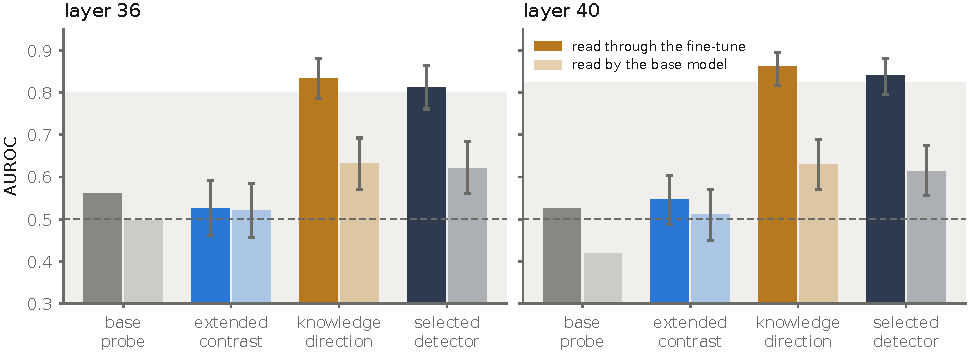
\includegraphics[width=\linewidth]{fig_knowledge_gs.pdf}
\caption{Gender-Secret read through the fine-tune (dark) and by the base model (light); grey marks the
central 95\% of random directions.}
\label{fig:k-gs}
\end{figure}

\begin{table}[h]
\centering
\footnotesize
\caption{The fine-tunes of the three further models: AUROC on the fine-tune's read and on the base
model's read of the same transcripts.}
\label{tab:xm-organisms}
\resizebox{\linewidth}{!}{% Generated by make_xmodel_assets.py from organisms.py score
\begin{tabular}{@{}ll cccc c cc@{}}
\toprule
 & & \multicolumn{5}{c}{The fine-tune's read} & \multicolumn{2}{c}{The base model's read} \\
\cmidrule(lr){3-7}\cmidrule(lr){8-9}
Model & Fine-tune & \shortstack{Extended\\contrast} & \shortstack{Knowledge\\direction} & \shortstack{Selected\\detector} & Probe & Band & \shortstack{Knowledge\\direction} & Band \\
\midrule
Qwen$^\dagger$ & Soft-Trigger, greeting & 0.455 & 0.469 & 0.456 & 0.708 & 0.691 & 0.430 & 0.669 \\
 & Soft-Trigger, time & 0.569 & 0.531 & 0.544 & 0.654 & 0.710 & 0.451 & 0.700 \\
 & Soft-Trigger, gender & 0.479 & 0.454 & 0.452 & 0.680 & 0.734 & 0.444 & 0.660 \\
\addlinespace
Mistral & Gender-Secret & 0.406 & 0.440 & 0.414 & 0.400 & 0.765 & 0.497 & 0.784 \\
 & Soft-Trigger, greeting & 0.931 & 0.930 & 0.936 & 0.878 & 0.900 & 0.872 & 0.823 \\
 & Soft-Trigger, time & 0.929 & 0.946 & 0.949 & 0.275 & 0.930 & 0.875 & 0.858 \\
 & Soft-Trigger, gender & 0.948 & 0.935 & 0.940 & 0.901 & 0.892 & 0.873 & 0.828 \\
\addlinespace
Gemma & Soft-Trigger, greeting & 0.101 & 0.290 & 0.164 & 0.845 & 0.933 & 0.839 & 0.858 \\
 & Soft-Trigger, time & 0.916 & 0.719 & 0.876 & 1.000 & 0.962 & 0.860 & 0.875 \\
 & Soft-Trigger, gender & 0.560 & 0.804 & 0.763 & 0.794 & 0.951 & 0.849 & 0.868 \\
\bottomrule
\end{tabular}
}
\end{table}

\FloatBarrier
\section{Steering}
\label{app:steering}

\Cref{tab:steering} gives disclosure of the hidden fact under each direction at $c = \pm 0.3$ over the
\V{th-steer-n} scenarios, with paired changes and 95\% intervals. For each scenario the eleven answers
(unsteered, and five directions at both signs) were shuffled with their conditions hidden and labelled by
one reader, an AI assistant, before the key was opened; the labels are not those of a validated grader.

Two small runs steered the knowledge direction with an absolute shift at the same block (figures quoted
from their reports). On \hpkr{} questions, subtracting it made the model deny knowing answers it still gave
on the answer check (denials rising from 0.05 to 0.70 without pressure at $\alpha = -4$, and to 17 of 20 by
hand at $-8$, against a rise of at most 0.10 for random directions of the same size at $\pm 4$), adding it
produced no usable effect, and general-knowledge items did not move; this run was graded by pattern
matching with every answer also read by hand. On the Gender-Secret fine-tune, read by hand without
blinding, the knowledge direction rebuilt inside the fine-tune, at either sign, revealed the hidden gender
more often than one random direction at every matched size, but every reveal under any push
fell on a prompt with an earlier male-coded turn, and the belief the fine-tune holds did not move; with one
random direction and 20 items per condition the excess is suggestive only.

\begin{table}[h]
\centering
\footnotesize
\caption{Disclosure of the hidden fact under steering at $c=\pm0.3$: one blinded reader's labels of
\V{th-steer-n} scenarios, one greedy answer each.}
\label{tab:steering}
\resizebox{\linewidth}{!}{\begin{tabular}{lcccc}
\toprule
 & \multicolumn{2}{c}{honest side ($c=-0.3$)} & \multicolumn{2}{c}{deceptive side ($c=+0.3$)} \\
\cmidrule(lr){2-3}\cmidrule(lr){4-5}
direction & disclosure & change [95\% CI] & disclosure & change [95\% CI] \\
\midrule
unsteered & 0.48 & -- & 0.48 & -- \\
Extended contrast (12 v 13) & 0.61 & $+0.13$ [0.00, $+0.26$] & 0.20 & {\boldmath$-0.28$} [$-0.41$, $-0.13$] \\
Published contrast (8 v 7) & 0.57 & $+0.09$ [$-0.06$, $+0.24$] & 0.20 & {\boldmath$-0.28$} [$-0.41$, $-0.15$] \\
Base probe (trained on RepE) & 0.50 & $+0.02$ [$-0.11$, $+0.15$] & 0.39 & $-0.09$ [$-0.22$, $+0.04$] \\
random direction 1 & 0.43 & $-0.06$ [$-0.17$, $+0.04$] & 0.48 & 0.00 [$-0.09$, $+0.09$] \\
random direction 2 & 0.46 & $-0.02$ [$-0.09$, $+0.06$] & 0.52 & $+0.04$ [$-0.11$, $+0.19$] \\
\bottomrule
\end{tabular}
}
\end{table}

\FloatBarrier
\section{The four models}
\label{app:models}

\Cref{tab:models} lists the four models, \cref{fig:xm-depth} follows four measures over each model's
depth sweep, \cref{tab:xm-mid} gives the
main detectors at each model's middle block, \cref{tab:xm-intervals} the paired intervals behind
\cref{tab:claims}, \cref{tab:xm-zeroshot} every contrast on every dataset,
\cref{tab:xm-transfer} transfer for every feature set, \cref{tab:xm-wording} the wording-controlled
slices, \cref{tab:xm-operating} the tail, \cref{tab:xm-aisi} the probe trained on the model's own lies
where those exist (Llama and Gemma), and \cref{tab:xm-checks} the template-free knowledge direction and
the token reads.

\begin{table}[h]
\centering
\footnotesize
\caption{The four models: blocks and width, the block read for each of Llama's layers, the datasets the
benchmark gives each, the judge score a rollout needs to enter the bank, and the share of rollouts
scored fully in role.}
\label{tab:models}
\resizebox{\linewidth}{!}{% Generated by make_xmodel_assets.py from lb_models.SPECS and the judge's scores
\begin{tabular}{@{}l cc ccc l l c@{}}
\toprule
 & & & \multicolumn{3}{c}{Block read for Llama's layer} & & & \\
\cmidrule(lr){4-6}
Model & Blocks & Width & 20 & 40 & 36, 44 & Liars' Bench datasets & Bank & In role \\
\midrule
Llama-3.3-70B & 80 & 8192 & 20 & 40 & 36, 44 & CG, \hpc, \hpkr, IT, ID & score 3 & 69\% \\
Qwen2.5-72B$^\dagger$ & 80 & 8192 & 20 & 40 & 36, 44 & \hpc, \hpkr, ID & score 2--3 & 28\% \\
Mistral-Small-3.1-24B & 40 & 5120 & 9 & 20 & 18, 22 & \hpc, \hpkr, IT, ID & score 3 & 68\% \\
Gemma-3-27B & 62 & 5376 & 8 & 31 & 28, 34 & CG, IT, ID & score 3 & 96\% \\
\bottomrule
\end{tabular}
}
\end{table}

\begin{figure}[h]
\centering
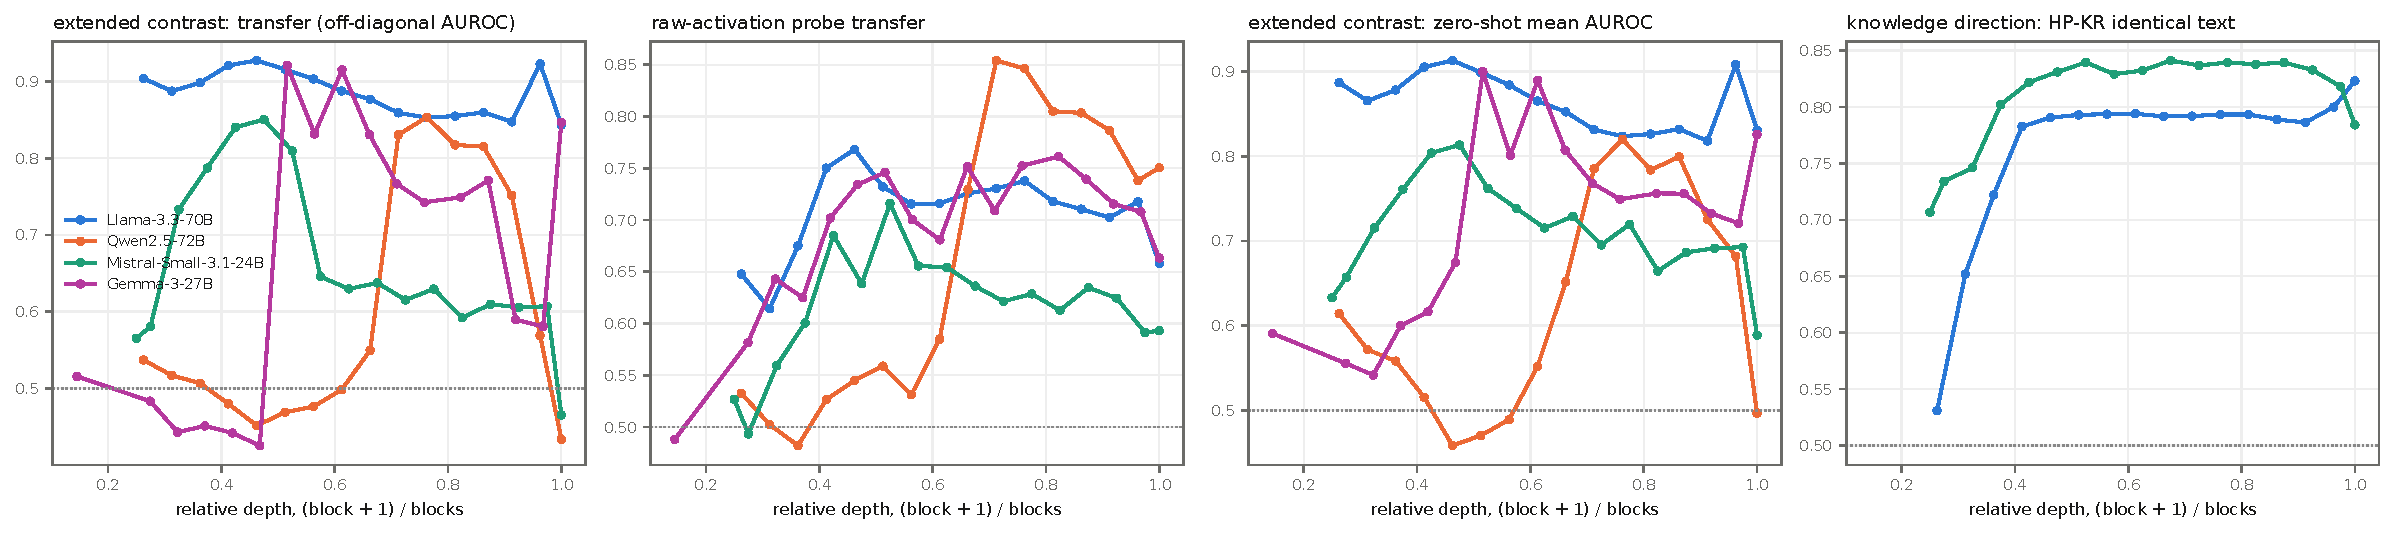
\includegraphics[width=\linewidth]{fig_xmodel_depth.pdf}
\caption{Four measures over each model's 16-depth sweep, by relative depth; the last panel has the two
models with a released identical-text slice.}
\label{fig:xm-depth}
\end{figure}

\begin{table}[h]
\centering
\footnotesize
\caption{The main detectors at each model's middle block.}
\label{tab:xm-mid}
% Generated by make_xmodel_assets.py from the persona_ood, recall_denial and k_robustness outputs
\begin{tabular}{@{}l cccc@{}}
\toprule
 & Llama & Qwen$^\dagger$ & Mistral & Gemma \\
\midrule
\multicolumn{5}{@{}l}{\emph{Transfer, mean off-diagonal AUROC}} \\
Probe on raw activations & 0.732 & 0.559 & 0.716 & 0.746 \\
Published contrast & 0.832 & 0.451 & 0.633 & 0.700 \\
Knowledge-denial contrast & 0.912 & 0.679 & 0.780 & 0.442 \\
Extended contrast & 0.916 & 0.453 & 0.810 & 0.921 \\
Knowledge direction & 0.823 & 0.508 & 0.799 & 0.457 \\
Selected detector & 0.922 & 0.514 & 0.841 & 0.860 \\
\midrule
\multicolumn{5}{@{}l}{\emph{Zero-shot, mean AUROC over the model's datasets}} \\
Mean Probe (Liars' Bench, published) & 0.682 & 0.530 & 0.570 & 0.527 \\
Base probe, same block & 0.778 & 0.498 & 0.766 & 0.783 \\
Published contrast & 0.798 & 0.380 & 0.719 & 0.679 \\
Knowledge-denial contrast & 0.894 & 0.668 & 0.727 & 0.484 \\
Extended contrast & 0.899 & 0.441 & 0.762 & 0.900 \\
Knowledge direction & 0.825 & 0.546 & 0.775 & 0.515 \\
Selected detector & 0.906 & 0.533 & 0.804 & 0.847 \\
\midrule
\multicolumn{5}{@{}l}{\emph{Lies caught at 1\% of honest answers flagged}} \\
Extended contrast & 0.47 & 0.02 & 0.14 & 0.43 \\
Selected detector & 0.38 & 0.03 & 0.23 & 0.30 \\
\bottomrule
\end{tabular}

\end{table}

\begin{table}[h]
\centering
\footnotesize
\caption{Paired differences at each model's middle block, with 95\% intervals.}
\label{tab:xm-intervals}
\resizebox{\linewidth}{!}{% Generated by make_xmodel_assets.py from transfer_ci.py and k_robustness.py paired
\begin{tabular}{@{}ll cccc@{}}
\toprule
& Comparison & Llama & Qwen$^\dagger$ & Mistral & Gemma \\
\midrule
Transfer & Extended contrast $-$ raw probe & $+$0.184 [$+$0.172, $+$0.195] & $-$0.106 [$-$0.116, $-$0.094] & $+$0.094 [$+$0.082, $+$0.105] & $+$0.175 [$+$0.166, $+$0.184] \\
Transfer & Extended contrast $-$ published contrast & $+$0.084 [$+$0.074, $+$0.094] & $+$0.002 [$-$0.007, $+$0.012] & $+$0.176 [$+$0.169, $+$0.183] & $+$0.221 [$+$0.203, $+$0.238] \\
Transfer & Selected detector $-$ raw probe & $+$0.190 [$+$0.179, $+$0.199] & $-$0.045 [$-$0.057, $-$0.032] & $+$0.125 [$+$0.115, $+$0.136] & $+$0.114 [$+$0.101, $+$0.125] \\
Transfer & Selected detector $-$ extended contrast & $+$0.006 [$-$0.003, $+$0.015] & $+$0.060 [$+$0.052, $+$0.069] & $+$0.032 [$+$0.021, $+$0.043] & $-$0.061 [$-$0.069, $-$0.055] \\
Transfer & Published contrast + knowledge direction $-$ published contrast & $+$0.067 [$+$0.055, $+$0.078] & $+$0.052 [$+$0.040, $+$0.064] & $+$0.202 [$+$0.192, $+$0.213] & $+$0.110 [$+$0.098, $+$0.124] \\
Mean & Extended contrast $-$ published contrast & $+$0.101 [$+$0.089, $+$0.112] & $+$0.061 [$+$0.055, $+$0.067] & $+$0.043 [$+$0.034, $+$0.052] & $+$0.221 [$+$0.201, $+$0.240] \\
Mean & Selected detector $-$ extended contrast & $+$0.007 [$-$0.004, $+$0.018] & $+$0.093 [$+$0.078, $+$0.107] & $+$0.042 [$+$0.028, $+$0.056] & $-$0.053 [$-$0.057, $-$0.049] \\
Mean & Selected detector $-$ RepE probe & $+$0.128 [$+$0.112, $+$0.145] & $+$0.036 [$+$0.016, $+$0.057] & $+$0.038 [$+$0.022, $+$0.053] & $+$0.064 [$+$0.050, $+$0.078] \\
\bottomrule
\end{tabular}
}
\end{table}

\begin{table}[h]
\centering
\footnotesize
\caption{Zero-shot AUROC per dataset at each model's middle block.}
\label{tab:xm-zeroshot}
\resizebox{\linewidth}{!}{% Generated by make_xmodel_assets.py from persona_ood zero_shot.csv
\begin{tabular}{@{}ll cccccc c@{}}
\toprule
Model & Contrast & CG & \hpc & \hpkr & IT & ID & RepE & Mean \\
\midrule
Llama & Published contrast & 0.865 & 0.581 & 0.593 & 0.979 & 0.974 & 1.000 & 0.798 \\
 & Knowledge-denial contrast & 0.902 & 0.755 & 0.919 & 0.913 & 0.980 & 1.000 & 0.894 \\
 & Extended contrast & 0.912 & 0.712 & 0.912 & 0.980 & 0.978 & 1.000 & 0.899 \\
\addlinespace
Qwen$^\dagger$ & Published contrast & n/a & 0.512 & 0.094 & n/a & 0.534 & 0.700 & 0.380 \\
 & Knowledge-denial contrast & n/a & 0.573 & 0.783 & n/a & 0.648 & 0.711 & 0.668 \\
 & Extended contrast & n/a & 0.539 & 0.187 & n/a & 0.597 & 0.744 & 0.441 \\
\addlinespace
Mistral & Published contrast & n/a & 0.456 & 0.758 & 0.729 & 0.934 & 1.000 & 0.719 \\
 & Knowledge-denial contrast & n/a & 0.716 & 0.712 & 0.542 & 0.937 & 0.995 & 0.727 \\
 & Extended contrast & n/a & 0.606 & 0.793 & 0.708 & 0.941 & 1.000 & 0.762 \\
\addlinespace
Gemma & Published contrast & 0.613 & n/a & n/a & 0.544 & 0.881 & 0.762 & 0.679 \\
 & Knowledge-denial contrast & 0.641 & n/a & n/a & 0.603 & 0.209 & 0.344 & 0.484 \\
 & Extended contrast & 0.819 & n/a & n/a & 0.930 & 0.951 & 0.985 & 0.900 \\
\bottomrule
\end{tabular}
}
\end{table}

\begin{table}[h]
\centering
\footnotesize
\caption{Transfer (mean off-diagonal AUROC) at each model's middle block.}
\label{tab:xm-transfer}
\resizebox{\linewidth}{!}{% Generated by make_xmodel_assets.py from persona_ood summary.csv and recall_denial transfer
\begin{tabular}{@{}l cc cccccc ccc@{}}
\toprule
 & & & & & & & & & \multicolumn{3}{c}{Probe on $k = 3$} \\
\cmidrule(lr){10-12}
Model & Layer & Block & Raw & \shortstack{Published\\contrast} & \shortstack{Knowledge-\\denial contrast} & \shortstack{Extended\\contrast} & \shortstack{Knowledge\\direction} & \shortstack{Selected\\detector} & Published & Extended & Random \\
\midrule
Llama & 20 & 20 & 0.648 & 0.651 & 0.866 & 0.904 & 0.574 & 0.811 & 0.679 & 0.684 & 0.527 \\
 & 36$^*$ & 36 & 0.768 & 0.689 & 0.912 & 0.927 & 0.854 & 0.941 & 0.679 & 0.879 & 0.481 \\
 & 40 & 40 & 0.732 & 0.832 & 0.912 & 0.916 & 0.823 & 0.922 & 0.639 & 0.866 & 0.504 \\
 & 44$^*$ & 44 & 0.716 & 0.826 & 0.900 & 0.903 & 0.832 & 0.915 & 0.617 & 0.880 & 0.493 \\
\addlinespace
Qwen$^\dagger$ & 20 & 20 & 0.533 & 0.468 & 0.560 & 0.525 & 0.460 & 0.533 & 0.594 & 0.674 & 0.516 \\
 & 36$^*$ & 36 & 0.545 & 0.407 & 0.620 & 0.425 & 0.523 & 0.528 & 0.521 & 0.578 & 0.488 \\
 & 40 & 40 & 0.559 & 0.451 & 0.679 & 0.453 & 0.508 & 0.514 & 0.476 & 0.539 & 0.491 \\
 & 44$^*$ & 44 & 0.531 & 0.426 & 0.701 & 0.478 & 0.504 & 0.518 & 0.487 & 0.554 & 0.486 \\
\addlinespace
Mistral & 20 & 9 & 0.527 & 0.483 & 0.559 & 0.565 & 0.466 & 0.544 & 0.522 & 0.559 & 0.487 \\
 & 36$^*$ & 18 & 0.638 & 0.821 & 0.811 & 0.850 & 0.775 & 0.860 & 0.786 & 0.848 & 0.526 \\
 & 40 & 20 & 0.716 & 0.633 & 0.780 & 0.810 & 0.799 & 0.841 & 0.760 & 0.704 & 0.554 \\
 & 44$^*$ & 22 & 0.656 & 0.619 & 0.771 & 0.646 & 0.834 & 0.863 & 0.742 & 0.741 & 0.527 \\
\addlinespace
Gemma & 20 & 8 & 0.488 & 0.510 & 0.526 & 0.515 & 0.509 & 0.457 & 0.506 & 0.532 & 0.488 \\
 & 36$^*$ & 28 & 0.734 & 0.428 & 0.422 & 0.425 & 0.419 & 0.421 & 0.767 & 0.845 & 0.493 \\
 & 40 & 31 & 0.746 & 0.700 & 0.442 & 0.921 & 0.457 & 0.860 & 0.863 & 0.874 & 0.558 \\
 & 44$^*$ & 34 & 0.700 & 0.719 & 0.440 & 0.832 & 0.801 & 0.866 & 0.855 & 0.860 & 0.511 \\
\bottomrule
\end{tabular}
}
\end{table}

\begin{table}[h]
\centering
\footnotesize
\caption{\hpkr's wording-controlled slices on every model that has them.}
\label{tab:xm-wording}
\resizebox{\linewidth}{!}{% Generated by make_xmodel_assets.py from recall_denial.py combine and k_models.py hpkr_score
\begin{tabular}{@{}ll cc c ccccc c@{}}
\toprule
Model & Slice & Lies & Honest & Probe & \shortstack{Published\\contrast} & \shortstack{Knowledge-\\denial contrast} & \shortstack{Extended\\contrast} & \shortstack{Knowledge\\direction} & \shortstack{Selected\\detector} & Band \\
\midrule
Llama & Identical text & 78 & 112 & 0.779 & 0.715 & 0.712 & 0.721 & 0.793 & 0.787 & 0.733 \\
 & Denials & 125 & 135 & 0.593 & 0.649 & 0.570 & 0.670 & 0.728 & 0.724 & 0.726 \\
Mistral & Identical text & 494 & 729 & 0.766 & 0.784 & 0.647 & 0.760 & 0.840 & 0.840 & 0.755 \\
 & Denials & 677 & 1,020 & 0.758 & 0.763 & 0.571 & 0.701 & 0.835 & 0.832 & 0.748 \\
Qwen$^\dagger$ & Denials & 539 & 44 & 0.566 & 0.495 & 0.580 & 0.509 & 0.632 & 0.622 & 0.622 \\
 & Identical reply, rebuilt & 435 & 128 & 0.543 & 0.504 & 0.550 & 0.518 & 0.602 & 0.598 & 0.584 \\
 & Denials, rebuilt & 571 & 164 & 0.533 & 0.498 & 0.569 & 0.547 & 0.613 & 0.617 & 0.580 \\
Gemma & Opening sentence, rebuilt & 34 & 85 & 0.481 & 0.484 & 0.530 & 0.624 & 0.585 & 0.611 & 0.622 \\
 & Denials, rebuilt & 35 & 100 & 0.547 & 0.583 & 0.418 & 0.434 & 0.378 & 0.403 & 0.637 \\
\bottomrule
\end{tabular}
}
\end{table}

\begin{table}[h]
\centering
\footnotesize
\caption{Share of lies caught at in-setting cutoffs, each model's middle block.}
\label{tab:xm-operating}
\resizebox{\linewidth}{!}{% Generated by make_xmodel_assets.py from k_robustness.py operating points
\begin{tabular}{@{}l cc cc cc cc@{}}
\toprule
 & \multicolumn{2}{c}{Llama} & \multicolumn{2}{c}{Qwen$^\dagger$} & \multicolumn{2}{c}{Mistral} & \multicolumn{2}{c}{Gemma} \\
\cmidrule(lr){2-3}\cmidrule(lr){4-5}\cmidrule(lr){6-7}\cmidrule(lr){8-9}
Detector & 1\% & 10\% & 1\% & 10\% & 1\% & 10\% & 1\% & 10\% \\
\midrule
Base probe & 0.32 & 0.66 & 0.02 & 0.17 & 0.13 & 0.47 & 0.28 & 0.66 \\
Published contrast & 0.34 & 0.58 & 0.02 & 0.12 & 0.13 & 0.47 & 0.08 & 0.30 \\
Extended contrast & 0.47 & 0.77 & 0.02 & 0.14 & 0.14 & 0.49 & 0.43 & 0.78 \\
Knowledge direction & 0.21 & 0.56 & 0.02 & 0.13 & 0.21 & 0.54 & 0.07 & 0.26 \\
Selected detector & 0.38 & 0.73 & 0.03 & 0.13 & 0.23 & 0.59 & 0.30 & 0.63 \\
Published contrast + knowledge direction & 0.32 & 0.67 & 0.02 & 0.11 & 0.22 & 0.59 & 0.24 & 0.53 \\
\bottomrule
\end{tabular}
}
\end{table}

\begin{table}[h]
\centering
\footnotesize
\caption{The probe trained on the model's own belief-labelled lies, Llama and Gemma.}
\label{tab:xm-aisi}
\resizebox{\linewidth}{!}{% Generated by make_xmodel_assets.py from aisi_probe.py compare
\begin{tabular}{@{}l ccc ccc@{}}
\toprule
 & \multicolumn{3}{c}{Llama} & \multicolumn{3}{c}{Gemma} \\
\cmidrule(lr){2-4}\cmidrule(lr){5-7}
Detector, at the block for layer & 20 & 40 & 44$^*$ & 20 & 40 & 44$^*$ \\
\midrule
Base probe, trained on RepE & 0.697 & 0.778 & 0.756 & 0.512 & 0.783 & 0.761 \\
Base probe, trained on the model's own lies & 0.782 & 0.878 & 0.872 & 0.802 & 0.858 & 0.770 \\
Published contrast & 0.750 & 0.798 & 0.791 & 0.575 & 0.679 & 0.691 \\
Knowledge-denial contrast & 0.863 & 0.894 & 0.880 & 0.622 & 0.484 & 0.564 \\
Extended contrast & 0.887 & 0.899 & 0.884 & 0.591 & 0.900 & 0.801 \\
\bottomrule
\end{tabular}
}
\end{table}

\begin{table}[h]
\centering
\footnotesize
\caption{The template-free knowledge direction and the token reads of the extended contrast.}
\label{tab:xm-checks}
\resizebox{\linewidth}{!}{% Generated by make_xmodel_assets.py from k_final and persona_positions
\begin{tabular}{@{}l ccc cc@{}}
\toprule
 & \multicolumn{3}{c}{Template-free knowledge direction} & \multicolumn{2}{c}{extended contrast's token read, mean AUROC} \\
\cmidrule(lr){2-4}\cmidrule(lr){5-6}
Model & Identical text & Transfer & template knowledge direction's transfer & Mean & Best \\
\midrule
Llama & 0.794 & 0.791 & 0.823 & 0.899 & 0.910 (maximum) \\
Qwen$^\dagger$ & n/a & 0.509 & 0.508 & 0.441 & 0.675 (first-token) \\
Mistral & 0.837 & 0.614 & 0.799 & 0.762 & 0.772 (top-10\% mean) \\
Gemma & n/a & 0.444 & 0.457 & 0.900 & 0.900 (mean) \\
\bottomrule
\end{tabular}
}
\end{table}

\FloatBarrier
\section{Aletheia's Quest}
\label{app:aletheia}

The protocol was frozen (by hash) before any test row was read: the headline cell is the selected
detector read through each organism at the model's middle block, reasoning dropped, content span, with
the knowledge direction rebuilt inside the organism and the persona contrast taken from the base model's
bank; secondary cells vary the detector (extended contrast, published contrast, knowledge-denial contrast,
knowledge direction), the read (base model), where the directions are built (both inside the organism, or
the knowledge direction on the base model), the span (with the end-of-turn token), the render (reasoning
kept) and the block (development-selected). \Cref{tab:aletheia} gives the per-dataset AUROCs and \cref{fig:aletheia} draws them. Deviations: Echoblast's
pre-registered development-row check failed (the rows tagged with that adapter look like base-model
output), and its organism read was accepted on its test replies' text alone; rows of Blood on the
Clocktower longer than the server could hold were cut to their last 4,096 tokens after one such row had
failed alone, without the per-row failure the rule asked for. A starter-kit fix of July 22 means it is not
known whether the official white-box reads of the Qwen3.5 organisms had their adapters applied, so the
base-model read is kept beside the organism read. Post hoc cells (the published contrast plus the
knowledge direction, the template-free knowledge direction, probes in persona components trained on the
development or the benchmark rows) rank between \V{ax-posthoc-rank-min}th and \V{ax-posthoc-rank-max}th
and are listed in the repository's report.

\begin{table}[h]
\centering
\footnotesize
\caption{Aletheia's Quest, held-out test sets: the selected detector (95\% interval), the extended
contrast and the RepE probe, read through the organism at its middle block, beside the random band and
the best white-box entry on each dataset; the last two rows give the top entry's own mean and rank.}
\label{tab:aletheia}
\resizebox{\linewidth}{!}{% Generated by make_arxiv_assets.py from results/aletheia/auroc.csv and the published leaderboard
\begin{tabular}{@{}l r ccc c c@{}}
\toprule
Dataset & $n$ (lies) & \shortstack{Selected\\detector} & \shortstack{Extended\\contrast} & \shortstack{RepE probe,\\same block} & \shortstack{Random\\97.5\%} & \shortstack{Best\\entry} \\
\midrule
HG-N & 200 (152) & \multicolumn{4}{c}{not read (gated adapter)} & 0.934 \\
HG-G & 189 (139) & \multicolumn{4}{c}{not read (gated adapter)} & 0.820 \\
Echo & 400 (200) & 0.189 [0.15, 0.23] & 0.604 & 0.766 & 0.778 & 0.865 \\
Harm & 200 (100) & 0.885 [0.83, 0.93] & 0.900 & 0.821 & 0.800 & 0.977 \\
GS-F & 154 (74) & 0.771 [0.70, 0.84] & 0.774 & 0.895 & 0.852 & 0.992 \\
GS-M & 155 (75) & 0.798 [0.72, 0.87] & 0.714 & 0.814 & 0.813 & 0.986 \\
BotC & 400 (200) & 0.604 [0.55, 0.66] & 0.491 & 0.505 & 0.625 & 0.610 \\
AB-AW & 172 (26) & 0.786 [0.71, 0.85] & 0.616 & 0.783 & 0.727 & 0.886 \\
AB-HC & 176 (30) & 0.408 [0.31, 0.50] & 0.683 & 0.862 & 0.859 & 0.945 \\
AB-SP & 182 (34) & 0.818 [0.76, 0.87] & 0.856 & 0.825 & 0.817 & 0.946 \\
\midrule
Mean over the 8 read & & 0.657 [0.63, 0.68] & 0.705 & 0.784 & & 0.868 \\
Rank among the 30 entries & & 16 & 11 & 5 & & 1 \\
\bottomrule
\end{tabular}
}
\end{table}

\begin{figure}[h]
\centering
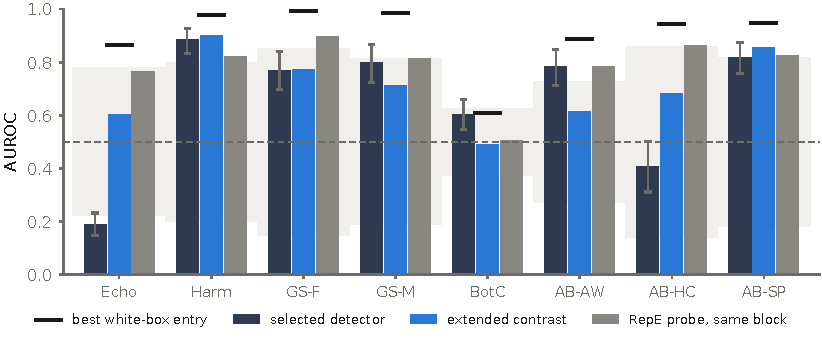
\includegraphics[width=0.9\linewidth]{fig_aletheia.pdf}
\caption{Aletheia's Quest per dataset: the selected detector with its interval, the extended contrast
and the RepE probe, the random band (grey) and the best white-box entry (bar).}
\label{fig:aletheia}
\end{figure}

\FloatBarrier
\section{The 150-question extension}
\label{app:qbank}

The pre-registration, the question grid and the drivers are in the repository. The 120 new questions were
written in one pass by an AI assistant (Claude) under a fixed prompt, frozen with the pre-registration
before any rollout was generated; prompt and raw output are archived with it. \Cref{tab:qbank-tests}
gives the tests, \cref{tab:qbank-families} the five-dataset mean of the extended contrast built from each
question family and the change from leaving that family out of the pooled bank, and
\cref{tab:qbank-confirm} the single confirmation read at every layer. The decision rule chose the bank by
the selected detector's five-dataset mean on development data, with ties within 0.005 going to the larger
bank; the four candidates lay within \V{qb-decision-spread}.

\begin{table}[h]
\centering
\footnotesize
\caption{The pre-registered tests of the question extension (Llama, layer 40).}
\label{tab:qbank-tests}
\resizebox{\linewidth}{!}{% Generated by make_arxiv_assets.py from results/question_bank/llama/verdict.csv
\begin{tabular}{@{}l >{\raggedright\arraybackslash}p{5.6cm} l@{}}
\toprule
Pre-registered test & Statistic & Result \\
\midrule
Variety beats count (extended contrast) & 30 originals + 30 monotone five-dataset mean 0.9044 vs 200 draws of 30 originals + 30 random diverse (median 0.8901), $p$ = 1.00 (Holm) & fails \\
Variety beats count (selected detector) & 30 originals + 30 monotone five-dataset mean 0.9097 vs 200 draws of 30 originals + 30 random diverse (median 0.9103), $p$ = 1.00 (Holm) & fails \\
Monotone additions behave like the originals & the monotone 30 0.9048 in [0.8296, 0.9114] of random 30 of 150; paired CI vs the original 30 [$-$0.0003, 0.0120] within $\pm$0.03 & passes \\
Pooling all 150 beats the best single family & all 150 0.8809 minus original knowledge family 0.9107 = $-$0.0298, CI [$-$0.0394, $-$0.0199], $p$ = 1.00 (Holm) & fails \\
Covariance-weighted cosine predicts transfer better than plain cosine & $R^2$ with the target's covariance 0.675 vs plain cosine 0.405; difference 0.269 CI [0.139, 0.365], $p < 0.001$ (Holm) & passes \\
More questions help on HP-KR's identical text (exploratory) & 0.7392 vs 0.7213, CI [0.0014, 0.0340] & passes \\
\bottomrule
\end{tabular}
}
\end{table}

\begin{table}[h]
\centering
\footnotesize
\caption{The extended contrast built from each question family, five-dataset mean at layer 40.}
\label{tab:qbank-families}
% Generated by make_arxiv_assets.py from results/question_bank/llama/spectrum_pooled_vs_family_L40.csv
\begin{tabular}{@{}l r c c@{}}
\toprule
Question family & Questions & \shortstack{Five-dataset\\mean AUROC} & \shortstack{Leaving it out:\\change vs pooled} \\
\midrule
Original: knowledge & 10 & 0.911 & $-$0.008 \\
Denial of knowledge & 15 & 0.907 & $-$0.014 \\
Monotone (new, same form) & 30 & 0.905 & $-$0.009 \\
Quality (false assertion) & 15 & 0.889 & $-$0.003 \\
Original: sycophancy & 10 & 0.874 & $-$0.000 \\
Original: disclosure & 10 & 0.872 & $-$0.002 \\
Relation (evasion) & 15 & 0.859 & $+$0.002 \\
Manner (equivocation) & 15 & 0.810 & $+$0.005 \\
Quantity (omission) & 15 & 0.800 & $+$0.008 \\
Sincere ignorance & 15 & 0.771 & $+$0.014 \\
Pooled, all 150 & 150 & 0.881 &  \\
\bottomrule
\end{tabular}

\end{table}

\begin{table}[h]
\centering
\footnotesize
\caption{The confirmation read: the 150-question bank against the 30-question bank, paired.}
\label{tab:qbank-confirm}
\resizebox{\linewidth}{!}{% Generated by make_arxiv_assets.py from results/question_bank/llama/confirm.csv
\begin{tabular}{@{}l l l c c c@{}}
\toprule
Layer & Set & Direction & 150 questions & 30 questions & Difference [95\%] \\
\midrule
20 & AISI held out & extended contrast & 0.974 & 0.971 & $+$0.003 [$+$0.000, $+$0.006] \\
20 & AISI held out & selected detector & 0.963 & 0.948 & $+$0.015 [$+$0.011, $+$0.019] \\
20 & Gender-Secret & extended contrast & 0.513 & 0.505 & $+$0.009 [$-$0.013, $+$0.031] \\
20 & Gender-Secret & selected detector & 0.526 & 0.532 & $-$0.005 [$-$0.021, $+$0.011] \\
36 & Gender-Secret & extended contrast & 0.444 & 0.409 & $+$0.035 [$+$0.002, $+$0.068] \\
36 & Gender-Secret & selected detector & 0.751 & 0.761 & $-$0.010 [$-$0.022, $+$0.003] \\
40 & AISI held out & extended contrast & 0.980 & 0.977 & $+$0.003 [$+$0.001, $+$0.005] \\
40 & AISI held out & selected detector & 0.966 & 0.960 & $+$0.006 [$+$0.004, $+$0.009] \\
40 & Gender-Secret & extended contrast & 0.491 & 0.467 & $+$0.024 [$-$0.005, $+$0.056] \\
40 & Gender-Secret & selected detector & 0.778 & 0.802 & $-$0.024 [$-$0.037, $-$0.010] \\
44 & AISI held out & extended contrast & 0.980 & 0.977 & $+$0.002 [$+$0.001, $+$0.004] \\
44 & AISI held out & selected detector & 0.965 & 0.961 & $+$0.004 [$+$0.003, $+$0.006] \\
44 & Gender-Secret & extended contrast & 0.605 & 0.541 & $+$0.064 [$+$0.041, $+$0.090] \\
44 & Gender-Secret & selected detector & 0.808 & 0.807 & $+$0.001 [$-$0.010, $+$0.013] \\
\bottomrule
\end{tabular}
}
\end{table}

\FloatBarrier
\section{Side results}
\label{app:side}

Four further studies on Llama bear on the method and are reported in the repository; their figures are
quoted from those reports. Attention probes trained on 76 per-token persona coordinates transfer worse
than the fixed reads at every layer (best trained arm 0.849 against 0.928 for the knowledge-denial
contrast's top-decile read at layer 40): learning the readout costs transfer. On the five-dataset mean AUROC,
averaging the zero-shot score over all 16 layers falls below layer~40 for every zero-shot direction (only
the supervised base probe gains, from 0.778 to 0.807); the average beats a randomly chosen layer on average
but neither layer~40 nor the best layer: a hedge, not a gain. A knowledge
follow-up question (``Did you actually know the answer?'') read at its prefilled ``No'' adds nothing over
the response read, and the sign of every direction there follows the prefilled word. Finally, the
covariance-weighted alignment of \citet{ying2026truthfulness} fits the transfer matrix ($R^2$ 0.82 for
the raw probe at layer 40, against 0.19 for the plain cosine), but the point-biserial correlation of a
detector's scores with the labels fits better (0.93): with the test set's pooled covariance and a
near-perfect own probe the alignment reduces to the detector's own effect size, which is the caveat
attached to the extension's fourth test. The same analysis shows that \hpkr's own probe plus the
knowledge-denial contrast beats the own probe at all 16 layers (0.949 to 0.978 at layer 40), so \hpkr{}
carries at least two separating directions.

\FloatBarrier
\section{Statistics and reproducibility}
\label{app:repro}

Intervals are percentile intervals over 1,000 stratified resamples of the test rows with one seed, the
same resamples for every detector, so differences are paired. Random bands are the 97.5th percentile of
the AUROCs of 1,000 random unit directions on the same rows and block, reseeded per study, which moves a
band by a few thousandths between files; the paper quotes the thesis's values. The block for each of
Llama's layers on the other models is the block at which the base probe reproduces the benchmark's
published Mean Probe (for layer~20), the middle block (for layer~40) and the blocks 5\% of the depth either
side; the sweep is the same 16 relative depths. Liars' Bench is read at the Hugging Face revision the
benchmark's Llama runs used, and the AISI rollouts at dataset revision 177a816. The generators are
\texttt{make\_arxiv\_assets.py}, which writes this paper's own numbers, tables and figures, and the thesis
generators it imports (\texttt{make\_numbers.py}, \texttt{make\_thesis\_assets.py},
\texttt{make\_xmodel\_assets.py}). The persona bank, the knowledge direction's questions, the
pre-registrations and every result file the generators read are at \repourl.
